\documentclass[runningheads,a4paper]{llncs}

\usepackage{amssymb}
\usepackage{wrapfig}
\setcounter{tocdepth}{3}
\usepackage{graphicx}
\usepackage{amsmath}
\usepackage{subfigure}
\usepackage{verbatim} 
\usepackage[hyphens]{url}
\usepackage{fixltx2e}
\usepackage{textcomp}
\usepackage{listings}
\lstset{
        basicstyle=\ttfamily\scriptsize,
        upquote=true,
        showspaces=false,
        showstringspaces=false,
        showtabs=false,
        tabsize=2,
        frame=none,
        breaklines,
        numbers=none,
        framexleftmargin=2mm,
        xleftmargin=2mm,
}

\usepackage{url}

\newcommand{\keywords}[1]{\par\addvspace\baselineskip
\noindent\keywordname\enspace\ignorespaces#1}

%% Define a new 'smallurl' style for the package that will use a smaller font.
\makeatletter
\def\url@smallurlstyle{%
  \@ifundefined{selectfont}{\def\UrlFont{\sf}}{\def\UrlFont{\scriptsize\ttfamily}}}
\makeatother
%% Now actually use the newly defined style.
\urlstyle{smallurl}
\newcommand{\nofootnote}[1]{~#1}

\begin{document}

\mainmatter  % start of an individual contribution

% first the title is needed
\title{A Tweet Consumers' Look At Twitter Trends}

% a short form should be given in case it is too long for the running head
\titlerunning{A Tweet Consumers' Look At Twitter Trends}
\authorrunning{A Tweet Consumers' Look At Twitter Trends}

\author{Thomas Steiner\inst{1} \and Arnaud Brousseau\inst{1,2}\thanks{The author is a graduate student at EURECOM, Sophia Antipolis (France), and currently works as an intern at Google Germany GmbH.} \and Rapha\"{e}l Troncy\inst{2}}

\institute{
  Google Germany GmbH, ABC-Str. 19, 20354 Hamburg, Germany\\ \email{\{tomac,arnaudb\}@google.com} \and
  EURECOM, Sophia Antipolis, France\\ \email{raphael.troncy@eurecom.fr}
}

\maketitle

\section{Introduction}\label{sec:introduction}
Twitter Trends allows for a global or local view on ``what's happening in my world right now" from a tweet producers' point of view. In this paper, we explore a way to complete Twitter Trends by having a closer look at the other side: the tweet consumers' point of view. While Twitter Trends works by analyzing the frequency of terms and their velocity of appearance in tweets being written, our approach is based on the popularity of extracted named entities in tweets being read.
 
\section{Twitter Swarm NLP Extension}\label{sec:twitterswarm}
We have developed a Google Chrome browser extension called Twitter Swarm NLP\footnote{\url{https://chrome.google.com/webstore/detail/dpbphenfafkflfmdlanimlemacankjol}} that injects JavaScript code into the Twitter.com homepage. The extension first checks if the user is logged in to Twitter.com, and if so, retrieves the tweets of the current user's timeline, search result page, or profile page, and performs named entity extraction via Natural Language Processing (NLP) using a remote NLP Web service\footnote{\url{http://tomayac.no.de/entity-extraction/combined/{text_to_be_analyzed}}} on each of the tweets. The extracted named entities are then displayed below each tweet, as can be seen in Figure \ref{fig:overtime-edge-a}. Finally the extracted named entities are sent to Google Analytics to compute trends by pivoting named entities by Analytics data, like users' geographic locations.

\section{Evaluation -- Raw Statistics}
We examined the period from February 24 to March 11, 2011. The extension reached \textit{1,009 pageviews} as reported by Analytics, and had \textit{35 all-time users} and \textit{28 seven-day active users}. All in all, the extension has detected \textit{1,533 unique different named entities} in total. 

Using Google Analytics, named entity occurrences can be easily tracked over time. As an example, Figure~\ref{fig:overtime-edge-b} shows the occurrences of the named entity ``tsunami". Japan was hit by an earthquake followed by a tsunami on March 11, exactly where the peak is on the graph. In general the occurrence graphs also for other examples indeed correspond to what we would expect, albeit the data is not statistically significant. One more example is ``iPad" with a peak on March 2, the release date of the iPad 2.

\begin{figure}[htb!]
  \begin{center}
\subfigure[Screenshot of a tweet, and a thereof extracted named entity ``gmail" with its representing DBpedia URI.]{\label{fig:overtime-edge-a}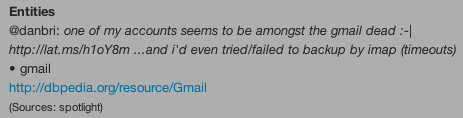
\includegraphics[width=0.495\linewidth]{danbri2.png}}
    \subfigure[Popularity of the named entity ``tsunami" over time (March 10 - 14). Japan was hit by a tsunami on March 11.]{\label{fig:overtime-edge-b}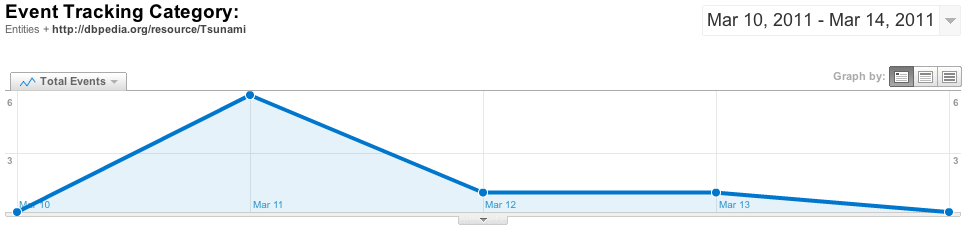
\includegraphics[width=0.495\linewidth]{tsunami.png}}
  \end{center}
  \caption{Twitter Swarm NLP sample output and popularity of a named entity over time.}
  \label{fig:overtime}
\end{figure}

\section{Evaluation -- Pivoting Named Entities By Country}
Japan was hit by an earthquake followed by a tsunami on March 11. Table~\ref{table:pivotbycountry} shows the occurrences distribution pivoted by country. Our data set is too small to be statistically significant, however, the potential for this data to reveal new insights is promising. Given enough data, we could, for example, provide an answer to the question whether among Twitter users the tsunami caused more interest in the American, or the European continent. As we use URIs as named entity identifiers, there is no ambiguity, and no language barriers, as we compare named entities on the level of the representing URIs, which are language-independent.

\begin{table}[htb!]
\begin{center}
\begin{tabular}{lllllllll}
\hline
Entity & Total & Germany & Finland & United States & Chile & India & Netherlands & Italy \\
\hline
\url{dbp:Tsunami} & 8 & 3 & 2 & 1 & 1 & 0 & 1 & 0 \\
\hline \\
\end{tabular}
\end{center}
\caption{The top named entity ``tsunami" (Mar. 10 - 14) pivoted by country.}
\label{table:pivotbycountry}
\end{table}

\section{Conclusion}\label{sec:conclusion}
In this paper, we measured the ``trendiness" of named entities in tweets being consumed using Google Analytics via an unobtrusive browser plug-in. This allows for even richer insights into, for example, the location of users interested in a certain named entity, sliceable back to any point (or period of time) in history where there is data available. This could be very attractive for market research.

%%%%%%%%%%%%%%%%%%%%%%
%%%  Bibliography  %%%
%%%%%%%%%%%%%%%%%%%%%%

\bibliographystyle{abbrv}
\bibliography{typeinst}

\end{document}